%==============================================================
%  Overlapping-Window Targets Manufacture Forecasting Skill
%  TMLR submission (anonymous). Compile (inline bibliography, no bibtex):
%    pdflatex paper && pdflatex paper
%==============================================================
\documentclass[10pt]{article}
% Numeric [n] citations, references after the appendices. For TMLR submission,
% delete the \PassOptionsToPackage and \setcitestyle lines to restore author-year.
\PassOptionsToPackage{numbers,sort&compress}{natbib}
\usepackage{tmlr}
\setcitestyle{numbers,square,citesep={,}}
% No running header ("Under review as submission to TMLR" removed).
\lhead{}
\renewcommand{\headrulewidth}{0pt}

\usepackage{amsmath,amssymb,amsfonts}
\usepackage{graphicx}
\graphicspath{{../figures/}{./}{figures/}}
\usepackage{booktabs}
\usepackage{array}
\usepackage{url}
\usepackage[hidelinks]{hyperref}
\usepackage{tikz}
\usetikzlibrary{positioning,arrows.meta}

\newcolumntype{L}[1]{>{\raggedright\arraybackslash}p{#1}}
\emergencystretch=2em

\title{Overlapping-Window Targets Manufacture Forecasting Skill:\\ Evidence from Trade Disruption Prediction}

% Hidden on anonymous TMLR submission; filled after acceptance.
\author{\name Anonymous Authors \email anonymous@openreview.net \\
\addr Anonymous Institution}

\def\month{09}
\def\year{2026}

\begin{document}

\maketitle

\begin{abstract}
Forecasting studies of supply chain and trade disruption report held-out skill without stating how much consecutive target values overlap and without a persistence baseline. We show on a four-year, 18-country monthly trade panel that when the target is built over a trailing window, that overlap, a bias long documented in financial econometrics, manufactures most of the reported skill. Writing the target as a window of $k$ one-step log returns, its lag-1 autocorrelation rises monotonically with the overlap fraction $(k-1)/k$, from $-0.449$ at zero overlap to $+0.677$ at eleven-twelfths, tracking from below the ceiling that overlap alone implies for independent increments. A rolling-median contraction target, whose consecutive values share eleven of twelve denominator months, is also positively autocorrelated ($+0.321$). On that target a zero-parameter persistence rule attains $R^2$ $0.648$ and is statistically tied with the strongest fitted models, a tuned ridge ($0.572$) and a converged graph network ($0.595$); on the non-overlapping one-step target the same rule is anti-predictive ($-1.909$), so model rankings invert. What survives is slight but decisively non-zero, and it is the target's own serial structure: an autoregression on its lags 1 and 12 reaches $R^2$ $0.215$, and on lag 1 alone $0.171$ (wild cluster bootstrap $p=0.001$ against zero, 17 clusters). Trade-volume features ($0.150$), a three-feature ridge ($0.138$), and graph networks ($0.077$ to $0.125$ over five seeds) beat neither (wild $p \ge 0.22$ against the one-lag model), and news, weather, and macro-stress channels add nothing measurable under either target. Persistence $R^2$ on the rolling-median target also swings from $-0.169$ to $+0.708$ across expanding-window origins with no parameters fitted. We document the corpus, target family, and protocol, and argue that stating a target's overlap and reporting a persistence baseline should be preconditions for reporting skill on this task.
\end{abstract}

%--------------------------------------------------------------
\section{Introduction}
\label{sec:intro}

Supply-chain risk papers now routinely report held-out skill on disruption targets, as precision, recall, and $F$-scores for late supplier deliveries~\citep{ref35,ref36}, accuracy and $F_1$~\citep{ref2,ref5}, or AUPRC~\citep{ref7}, and some grade disruption as a deviation from a reference level, such as a percentage capacity reduction~\citep{ref23}. None of the works we reviewed states how much consecutive target values overlap, and none reports a last-period persistence baseline (Section~\ref{sec:related}). That combination is enough to manufacture an appearance of skill: when a target overlaps its own lag and no baseline can exploit the overlap, the construction's contribution is credited to the model. The same construction is a known source of spurious long-horizon $R^2$ in financial econometrics~\citep{ref29,ref30,ref31,ref32}. The mechanism is known. What this paper adds is its measurement on a panel built from public trade data, and evidence that the correction has not reached this literature.

Let $V_t$ be inbound trade and $r_t=\log(V_t/V_{t-1})$ the one-step log return. A $k$-month window $H_k=\log(V_{T+1}/V_{T-k+1})$ is the sum of $k$ consecutive increments. Consecutive windows share $k-1$ of those $k$ increments, so the mechanical lag-1 autocorrelation for independent increments is $(k-1)/k$. Rolling-median contraction, the target this corpus originally used, is the same construction in different clothing: consecutive months share $11/12$ of a slow denominator.

On an 18-country monthly panel for 2021--2024, lag-1 autocorrelation of $H_k$ rises monotonically from $-0.449$ at $k=1$ to $+0.677$ at $k=12$, always below the $(k-1)/k$ ceiling, with a gap that narrows as $k$ grows because negatively autocorrelated increments are averaged out (Fig.~\ref{fig:overlap}). A zero-parameter persistence rule tracks the same curve. Once the overlap is removed, the best models use only the target's own history: a univariate AR(1) reaches $R^2=0.171$, and adding the twelve-month lag lifts it to $0.215$. Every engineered addition (trade-volume features, exogenous news, weather and macro channels, snapshot GCNs, temporal graph networks) scores lower.

Four contributions follow.
\begin{enumerate}
\item \textbf{Measurement of a known bias on this task.} We import the overlapping-observations correction from financial econometrics~\citep{ref29,ref32}, state overlap fractions for a target family $H_k$, and show that apparent skill tracks the $(k-1)/k$ ceiling on a panel built from public trade data (Finding F1).
\item \textbf{A rank corollary.} Persistence is top-tier under overlap and anti-predictive without it, so model rankings that omit a persistence baseline can order predictors backwards (F2).
\item \textbf{A documented corpus and protocol.} Forward-chained split, train-only transforms, matched-compute graph training, and Diebold--Mariano plus cluster-bootstrap tests~\citep{ref28,ref33,ref34}.
\item \textbf{An exogenous and architectural null.} News, weather, GSCPI, and graph structure add nothing measurable beyond the target's own lags (F3, F4). Single-split evaluation reports regime (F5).
\end{enumerate}

We do not claim a deployed extraction system. A LangGraph pipeline exists for live scoring; its LLM extractors are unvalidated, so every number below measures the fused historical corpus, not the live agents (Section~\ref{sec:limits}).

\section{Related Work}
\label{sec:related}

Table~\ref{tab:litsynth} (Appendix~\ref{app:lit}) maps the adjacent literature. We retarget the synthesis around three reporting questions, not around model class.

\paragraph{Who reports a persistence (or other naive) baseline?}
Almost nobody in Table~\ref{tab:litsynth} reports one that could exploit a target's memory. The two industrial delivery-delay case studies compare against class-prior rules: \citet{ref35} against the majority-class ``Zero Rule'', and \citet{ref36} against random and prevalence-weighted guessing. \citet{ref2} compares one ensemble against logistic regression, an SVM, a random forest, XGBoost, and a DNN; \citet{ref5} drops the graph but keeps an MLP; \citet{ref7} report AUPRC against learned graph and meta-learning baselines. The nearest thing to a naive floor is an ARMA baseline in \citet{ref6}. A last-period copy of the target is absent. On an overlapping target the omission matters, because persistence reads the window out mechanically. The dynamic-graph literature has met a version of the same issue: \citet{ref14} point out that a memorisation baseline built from past edges alone can be competitive, and argue that current benchmark datasets may be too simple to tell models apart.

\paragraph{Who states the target's overlap structure?}
The overlapping-observations problem is established in financial econometrics. \citet{ref29} showed that sampling more finely than the forecast horizon induces serial correlation that invalidates ordinary inference. \citet{ref30} showed that the usual asymptotic distributions approximate statistics computed from multiyear overlapping returns poorly, and derived an alternative theory. \citet{ref31} showed that rolling summation of $I(0)$ series produces long-horizon $R^2$ and $t$-statistics that do not have the usual limiting distributions, so long-horizon regressions can look significant whether or not a structural relation exists. \citet{ref32} showed that overlapping returns plus persistent regressors make estimated coefficients and $R^2$ grow with the horizon even when returns are unpredictable, which is mechanical long-horizon skill.

Deviation-from-baseline labels appear in disruption scoring: \citet{ref23} grade disruption severity by percentage capacity reduction, while other entries use annotated risk-event labels~\citep{ref7} or forecast shipment and congestion levels directly~\citep{ref17}. Evaluation splits are often not forward-chained either: \citet{ref35} hold out a random 20\% of six years of dated deliveries, \citet{ref16} use a random 7:1:2 split, and \citet{ref36} do not describe a split. We did not find a paper in Table~\ref{tab:litsynth} that reports the fraction of months shared between consecutive target values, or the implied autocorrelation ceiling $(k-1)/k$. The finance correction has not been imported as a reporting floor for trade-disruption forecasts. Section~\ref{sec:results} measures its size on this panel.

\paragraph{Who ablates exogenous channels against an autoregressive control?}
News and weather channels are motivated in this literature: \citet{ref21} classify supply-chain risk from news articles with an LLM, and \citet{ref17} condition disruption control on typhoon tracks. Ablations typically strip the graph~\citep{ref5,ref7} rather than asking whether the non-trade channels beat a lagged target. Section~\ref{sec:results} does that, after re-engineering each channel from its raw source.

Graph architectures remain relevant as a \emph{negative} test. Snapshot GCNs and TGNs~\citep{ref10,ref13} are the natural candidates once the panel is a country graph with monthly events. \citet{ref10} define the TGN internals we reuse, and describe TGAT~\citep{ref13} as the special case of TGN without memory; we do not re-derive them. When \citet{ref11} reran established dynamic-graph baselines in one standardised library, several did not reproduce their published scores, which the authors suggest reflects uneven implementations. Section~\ref{sec:results} finds the same sensitivity to protocol in single-seed graph runs. Continuous-time models have not been scored on public trade-disruption targets. Our result is that, at matched compute, they do not beat even a univariate AR(1) once overlap is removed.

%--------------------------------------------------------------
\section{Corpus and Targets}
\label{sec:corpus}

Figure~\ref{fig:pipeline} summarises the pipeline from raw sources to the significance tests. Every stage runs on frozen files; nothing in it touches the live system of Section~\ref{sec:limits}.

\begin{figure}[t]
\centering
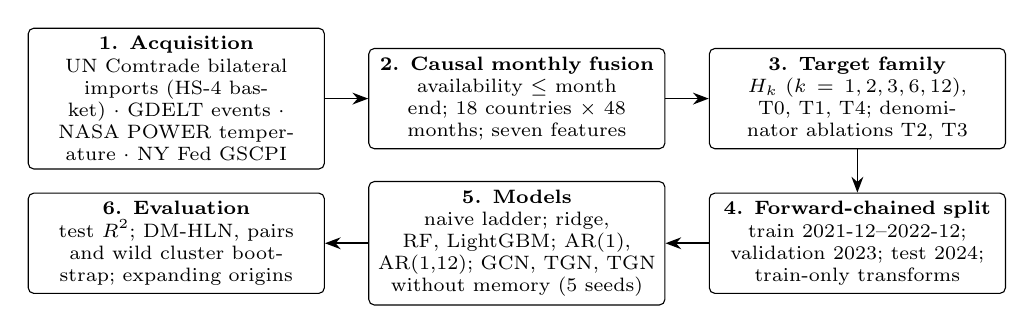
\begin{tikzpicture}[
  box/.style={draw, rounded corners=2pt, align=center, font=\scriptsize,
              minimum height=1.25cm, text width=3.55cm, inner sep=3pt},
  arr/.style={-{Stealth[length=2mm]}, semithick},
  node distance=0.55cm and 0.55cm]
\node[box] (src) {\textbf{1. Acquisition}\\ UN Comtrade bilateral imports (HS-4 basket) $\cdot$ GDELT events $\cdot$ NASA POWER temperature $\cdot$ NY Fed GSCPI};
\node[box, right=of src] (fuse) {\textbf{2. Causal monthly fusion}\\ availability $\le$ month end; 18 countries $\times$ 48 months; seven features};
\node[box, right=of fuse] (tgt) {\textbf{3. Target family}\\ $H_k$ ($k=1,2,3,6,12$), T0, T1, T4; denominator ablations T2, T3};
\node[box, below=of tgt] (split) {\textbf{4. Forward-chained split}\\ train 2021-12--2022-12; validation 2023; test 2024; train-only transforms};
\node[box, left=of split] (mod) {\textbf{5. Models}\\ naive ladder; ridge, RF, LightGBM; AR(1), AR(1,12); GCN, TGN, TGN without memory (5 seeds)};
\node[box, left=of mod] (inf) {\textbf{6. Evaluation}\\ test $R^2$; DM-HLN, pairs and wild cluster bootstrap; expanding origins};
\draw[arr] (src) -- (fuse);
\draw[arr] (fuse) -- (tgt);
\draw[arr] (tgt) -- (split);
\draw[arr] (split) -- (mod);
\draw[arr] (mod) -- (inf);
\end{tikzpicture}
\caption{Pipeline. Stages 1--2 build the corpus (Section~\ref{sec:corpus}); stages 3--6 are the protocol (Sections~\ref{sec:protocol}--\ref{sec:models}).}
\label{fig:pipeline}
\end{figure}

\paragraph{Data acquisition.}
The unit is a country $\times$ month: 18 countries, 48 months (2021-01 through 2024-12), 864 rows. Four public sources are used (Table~\ref{tab:sources}). Trade comes from UN Comtrade monthly bilateral import records (flow code M) for an eleven-code HS-4 consumer-goods basket: 8517, 8471, 8528, 8516, 8507, 9403, 6109, 6203, 6204, 9503, and 3304. The country universe fixes India and adds India's largest partners in this basket that also report import data to Comtrade, which yields 18 countries. Each Comtrade record keeps its publication date. News comes from the GDELT daily event files, restricted to events whose CAMEO root code is 14 or 16--19 (protest, reduced relations, coercion, assault, fighting) and in which a panel country is an actor. Daily temperature comes from NASA POWER at a representative coordinate for each country, and global supply-chain stress from the monthly New York Fed Global Supply Chain Pressure Index (GSCPI).

\begin{table}[t]
\centering
\caption{Data sources. All four are public; the corpus redistributes only the fused country-month table.}
\label{tab:sources}
\footnotesize
\begin{tabular}{l l l l}
\toprule
\textbf{Source} & \textbf{Content} & \textbf{Resolution} & \textbf{Used as} \\
\midrule
UN Comtrade & bilateral imports, HS-4 basket & monthly, country pair & $V_{v,t}$, targets, flow proxies, graph edges \\
GDELT & CAMEO-coded news events & daily events & news volume, negative tone, strike flag \\
NASA POWER & 2 m air temperature & daily, per country & weather flag; seasonal temperature $z$ \\
NY Fed GSCPI & global supply-chain pressure & monthly, global & global stress level and its change \\
\bottomrule
\end{tabular}
\end{table}

\paragraph{Causal monthly fusion.}
Sources are fused into one row per country and month. A feature for month $T$ uses only observations whose reference date and availability date both fall on or before the last day of $T$, so a 2024 test month cannot see a later Comtrade revision or a late-arriving event. Inbound flow $V_{v,t}$ is the basket value country $v$ imports from the other panel countries in month $t$. Let $q_{v,t}=V_{v,t}/\tilde V_{v,t}$ be the flow ratio, where $\tilde V_{v,t}$ is the median of the previous three months. Each row carries seven features: an inventory proxy $30\,\min\{\max(q_{v,t},1/6),3\}$; a delay proxy $30\max(0,1-q_{v,t})$; news volume, the count of matching events added in the trailing seven days; the share of events in the trailing three days with average tone at or below $-2$; a strike flag, set when any labour-unrest event (CAMEO base code 143 or 144) becomes available during the month; a weather flag, set when any daily temperature in the trailing seven days deviates from that week's mean by more than 1.5 standard deviations; and the latest published GSCPI value. All four sources cover all 18 countries; GDELT publishes no daily file for two dates (2022-11-10 and 2023-03-23), which are skipped.
\paragraph{Split.}
Forward-chained: train 2021-12--2022-12, validation 2023, test 2024-01--2024-11. Training starts in December 2021 because the twelve-month median behind T0 and its lag needs the preceding eleven months. December 2024 is dropped from the test window because every target is dated at $T+1$ and no January 2025 flow is observed, which leaves $18\times11=198$ test country-months; after rows with zero or missing flow are removed, the test fold has $n=193$ with a valid T0 label and $n=187$ with a valid T1 log return. The training fold has 234 country-months and the validation fold 216 (T0) or 215 (T1). All scalers and graph edge scales are fit on training months only; hyperparameters are selected on the validation year. We write ``test 2024'' throughout for this eleven-month fold.

\paragraph{Target family.}
Let $V_{v,t}$ be inbound flow of country $v$ in month $t$, and $r_{v,t}=\log(V_{v,t}/V_{v,t-1})$ when both are positive. Table~\ref{tab:targets} defines the targets. $H_k=\log(V_{T+1}/V_{T-k+1})$ is an overlapping sum of $k$ increments; $H_1$ is T1 and $H_{12}$ is T4. T0 is rolling-median contraction, the original paper target. T2 (constant per-country denominator) and T3 (disjoint feature denominator) isolate which piece of T0 carries the artifact: T2 holds because the numerator is still a level; T3 holds because it changes a feature, not the mean-reverting target (Table~\ref{tab:t2t3}, Appendix~\ref{app:t2t3}).

We report regression only. A prevalence-matched binary label on the T1 log return under-fires on 2024 (10 positives), too few to support a classification claim.

\begin{table}[t]
\centering
\caption{Target family, and the whole of F1 in one table. Overlap is the fraction of months (or increments) shared with the lag-1 value; for independent increments it is \emph{also} the mechanical lag-1 autocorrelation ceiling, so the Overlap column doubles as the ceiling and Gap $=$ Overlap $-$ AC. Lag-1 AC is within-country, pooled. Persistence is the zero-parameter rule $\hat{y}_T=y_{T-1}$, scored two ways: averaged over expanding origins (Table~\ref{tab:origins}) and on the 2024 test fold alone. AC and origin-mean persistence rise monotonically with overlap; the single-fold column dips at $k=3$, which is why Fig.~\ref{fig:overlap} plots the origin-mean. Source: \texttt{results/phase06/horizon\_sweep.csv}.}
\label{tab:targets}
\footnotesize
\begin{tabular}{l l c c c c c}
\toprule
& & \textbf{Overlap} & \textbf{Lag-1} & & \multicolumn{2}{c}{\textbf{Persistence $R^2$}} \\
\cmidrule(l){6-7}
\textbf{Id} & \textbf{Definition} & \textbf{(=ceiling)} & \textbf{AC} & \textbf{Gap} & \textbf{origin-mean} & \textbf{2024} \\
\midrule
T1 $=H_1$ & $\log(V_{T+1}/V_T)$ & $0$ & $-0.449$ & $0.449$ & $-1.744$ & $-1.909$ \\
$H_2$ & $\log(V_{T+1}/V_{T-1})$ & $1/2$ & $+0.056$ & $0.444$ & $-0.748$ & $-0.349$ \\
$H_3$ & $\log(V_{T+1}/V_{T-2})$ & $2/3$ & $+0.195$ & $0.472$ & $-0.364$ & $-0.528$ \\
$H_6$ & $\log(V_{T+1}/V_{T-5})$ & $5/6$ & $+0.493$ & $0.340$ & $-0.228$ & $+0.098$ \\
T4 $=H_{12}$ & $\log(V_{T+1}/V_{T-11})$ & $11/12$ & $+0.677$ & $0.240$ & $+0.311$ & $+0.489$ \\
T0 & $(V_{T+1}-\mathrm{med}_{12})/\mathrm{med}_{12}$ & $\approx 11/12$ den. & $+0.321$ & --- & $+0.172$ & $+0.648$ \\
\bottomrule
\end{tabular}
\end{table}

%--------------------------------------------------------------
\section{Protocol}
\label{sec:protocol}

\paragraph{Baseline ladder.}
Zero, persistence ($c_{T-1}$), seasonal ($c_{T-11}$), per-country training median, global training median, then fitted models. Persistence is the quantity the overlap mechanism predicts; omitting it is what lets overlapping targets look like model skill. Table~\ref{tab:ladder} reports the full ladder on all three targets. We print it because it is the reporting floor this paper argues for, and because applying that floor to our own earlier draft is what produced F2: the seven-feature ridge of an earlier version of this work scores $R^2=0.378$ on T0 but $-0.032$ on the overlap-free target, below the zero baseline.

\begin{table}[t]
\centering
\caption{The prescribed reporting floor, applied to this panel: full baseline ladder plus fitted tabular models, test 2024 $R^2$, on the rolling-median target (T0), the overlap-free target (T1), and the twelve-month overlapping window (T4). This is not a leaderboard; the informative rows are the naive ones. Persistence needs zero parameters and moves from best-in-table on T0 to far below zero on T1, tracking overlap (Table~\ref{tab:targets}), while the seven-feature ridge of the earlier draft goes from $0.378$ to $-0.032$. Graph models at matched compute are in Table~\ref{tab:ranks}. Source: \texttt{results/canonical\_numbers.csv}.}
\label{tab:ladder}
\footnotesize
\begin{tabular}{l l ccc}
\toprule
& & \textbf{T0} & \textbf{T1} & \textbf{T4} \\
\textbf{Model} & \textbf{Params} & (ovl.\ $\approx 11/12$) & (ovl.\ $0$) & (ovl.\ $11/12$) \\
\midrule
Zero & $0$ & $-0.007$ & $-0.000$ & $-0.013$ \\
Persistence $c_{T-1}$ & $0$ & $\mathbf{0.648}$ & $-1.909$ & $0.489$ \\
Seasonal $c_{T-11}$ & $0$ & $-0.437$ & $-1.648$ & $-1.467$ \\
Per-country median & $0$ & $-0.302$ & $-0.078$ & $-1.329$ \\
Global median & $0$ & $-0.090$ & $-0.008$ & $-0.541$ \\
\midrule
Ridge, original 7 feat. & fitted & $0.378$ & $-0.032$ & $-0.128$ \\
Random forest & fitted & $0.280$ & $0.118$ & $0.287$ \\
LightGBM & fitted & $0.233$ & $0.033$ & $0.300$ \\
AR ridge, 3 feat. & fitted & $0.572$ & $0.138$ & $0.273$ \\
Univariate AR(1) & fitted & $0.567$ & $\mathbf{0.171}$ & $0.416$ \\
\bottomrule
\end{tabular}
\end{table}

\paragraph{Selection.}
Hyperparameters (ridge $\alpha$, tree depth, LightGBM leaves) are chosen on 2023 validation $R^2$ and reported once on 2024. Graph models: 80 epochs, patience 15, five seeds, best-validation epoch, identical budget across GCN, TGN, and TGN-without-memory.

\paragraph{Inference.}
Squared-error Diebold--Mariano~\citep{ref28} with the Harvey--Leybourne--Newbold small-sample correction~\citep{ref33}, plus a country-clustered pairs bootstrap and a wild cluster bootstrap with Rademacher weights (9{,}999 replications, null imposed)~\citep{ref34}. The unit is country$\times$month; there are 18 country clusters under T0 and 17 under T1 (one country has no valid log return in 2024). Seventeen or eighteen is few: we treat the wild bootstrap as load-bearing; DM-HLN is misspecified for a panel and the pairs bootstrap over-rejects with few clusters~\citep{ref34}. Tests are unadjusted for multiplicity. Graph $R^2$ in Table~\ref{tab:ranks} reports both the mean of five seed-wise scores and the $R^2$ of the seed-averaged prediction used in the Diebold--Mariano tests. Seed averaging lifts GCN from $0.077$ to $0.119$ on T1, consistent with its higher seed variance; the ensemble still does not reach the univariate AR(1) at $0.171$.

\paragraph{Metric.}
Skill is out-of-sample $R^2=1-\sum(y-\hat y)^2/\sum(y-\bar y)^2$ on the test fold, with $\bar y$ the test-fold mean; this is why the zero predictor scores slightly below zero. All results are regression; no classification result is reported.

%--------------------------------------------------------------
\section{Models}
\label{sec:models}

Tabular: ridge, random forest, LightGBM on either the original seven features (inventory and delay proxies, news volume, negative tone, strike flag, weather flag, GSCPI) or the three-feature AR set (the clipped flow ratio $\min\{\max(q_{v,t},1/6),3\}$ of Section~\ref{sec:corpus}, the T0 lag, and the flow-ratio lag). The univariate AR(1) uses only the target's own lag; the AR(1,12) adds the target's value twelve months earlier. Both are ridge regressions with $\alpha$ selected on validation.

Graphs reuse the repository heads: a two-layer snapshot GCN and a TGN with 32-dimensional memory~\citep{ref10}, plus a TGN with memory disabled. Each month is a graph on the 18 countries whose edges are the observed bilateral Comtrade flows among them (about 600 records per month). The GCN uses the symmetrised edge set; the TGN consumes each month's edges as events carrying two edge features, log trade value (scaled by its training-window maximum) and log volume. Node features are the three AR features, standardized on train. We do not claim architectural novelty.

%--------------------------------------------------------------
\section{Results}
\label{sec:results}

\subsection{F1. Overlap manufactures skill}

F1's mechanism is the overlapping-observations bias of \citet{ref29}, \citet{ref30}, \citet{ref31}, and \citet{ref32}: consecutive long-horizon windows share increments, so serial correlation and $R^2$ rise with horizon under the null. That correction has not been applied to trade-disruption forecasts. Fig.~\ref{fig:overlap} measures its size on this panel. Lag-1 autocorrelation of $H_k$ and origin-mean persistence $R^2$ both rise with overlap fraction $(k-1)/k$. Autocorrelation stays below the i.i.d.\ ceiling at every $k$. The gap is $0.45$ for $k\le 3$ and narrows to $0.24$ at $k=12$: as the window widens, increment-level negative correlation is a smaller share of the sum's variance, so observed AC approaches the ceiling from below. T1 increments themselves carry positive longer-lag memory: lag-2 $+0.044$, lag-3 $+0.107$, and, most relevantly for the twelve-month window, lag-6 $+0.287$ and lag-12 $+0.294$ (within-country, pooled). The residual gap at large $k$ is therefore measured structure, not a free parameter. The annual terms are the largest, which is why the gap closes fastest exactly where the window starts to span a year. T0 is not an $H_k$ window, but consecutive T0 values share eleven of twelve denominator months, and T0 is likewise positively autocorrelated (AC $+0.321$). Table~\ref{tab:targets} gives the full sweep.

A closed-form MA(1) overlapping-sum autocorrelation, substituting $\rho=-0.449$, underpredicts at high $k$ ($0.53$ vs $0.68$ at $k=12$). We do not overlay it. The directional claim does not need it: skill is a monotone function of a quantity you can write down before fitting any model.

\begin{figure}[t]
\centering
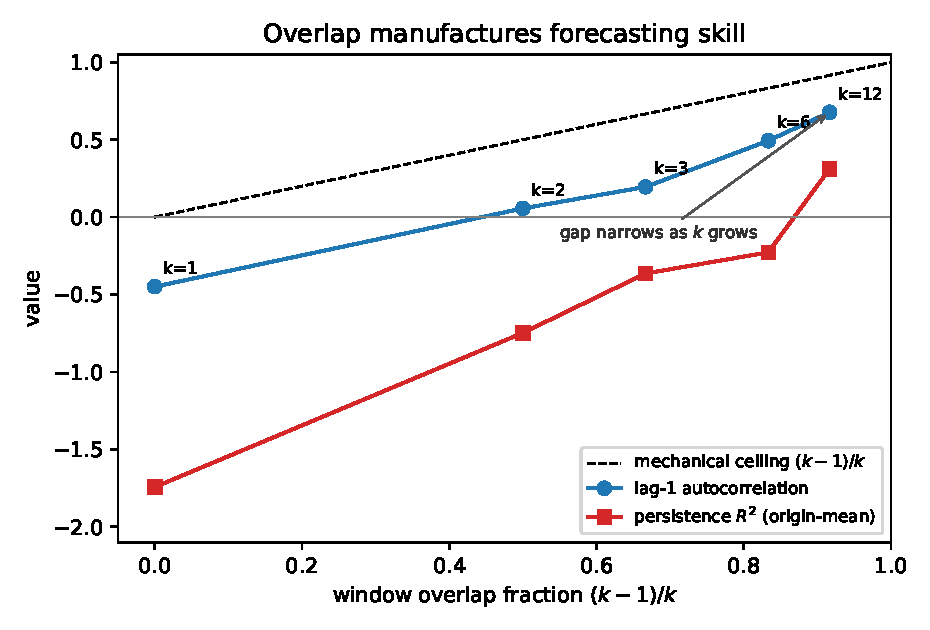
\includegraphics[width=\columnwidth]{overlap_vs_skill.pdf}
\caption{Overlap fraction $(k-1)/k$ versus lag-1 autocorrelation of $H_k$ and origin-mean persistence $R^2$. Dashed line: i.i.d.\ mechanical ceiling. Persistence scored on the single 2024 test fold alone is omitted from the plot (non-monotone at $k=3$, $n=187$); it is reported in Table~\ref{tab:targets} and in the accompanying CSV.}
\label{fig:overlap}
\end{figure}

\subsection{F2. Rankings invert (corollary of F1)}

Because T1 increments are negatively autocorrelated, a persistence rule (coefficient fixed at $+1$) is anti-predictive on T1 ($R^2=-1.909$) while a fitted AR(1) scores $0.171$ precisely because it learns a negative coefficient ($-0.055$ on the train-standardized lag). On T0 the same persistence rule is top-tier ($0.648$) and statistically tied with the strongest fitted models (wild $p=0.778$ vs the GCN ensemble, $0.986$ vs the tuned ridge). The size of the T1 collapse is what theory predicts: for a stationary series with lag-1 autocorrelation $\rho_1$, persistence has population $R^2=1-2(1-\rho_1)=2\rho_1-1$, so $\rho_1=-0.449$ implies $-1.90$, against $-1.909$ observed. Table~\ref{tab:ranks} is the rank comparison at matched budget; Table~\ref{tab:ladder} shows that the inversion runs through the entire naive ladder, not just persistence, and Fig.~\ref{fig:rank} draws that ladder on both targets. The inversion is therefore a consequence of F1 together with $\rho_1(H_1)<0$, not a separate finding.

\begin{figure}[t]
\centering
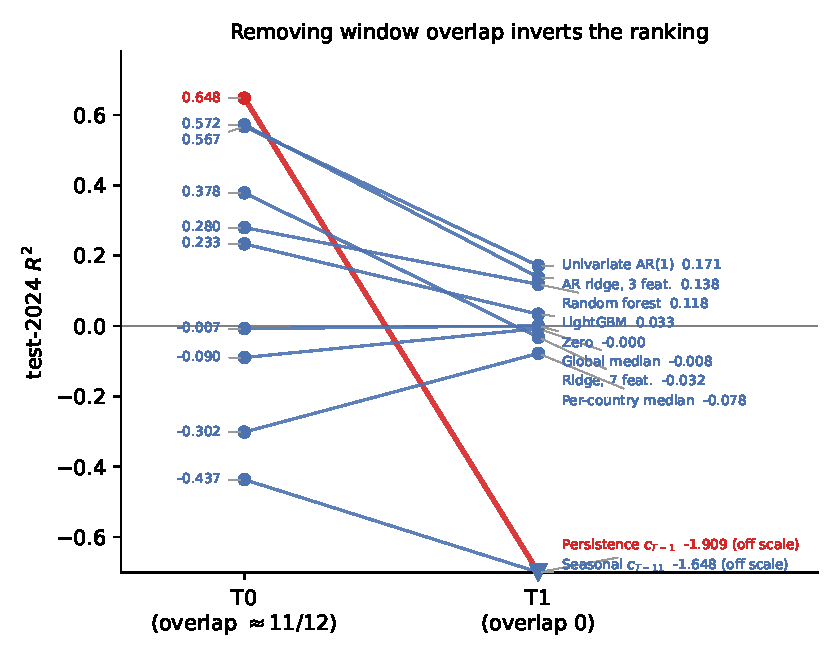
\includegraphics[width=0.8\columnwidth]{rank_inversion.pdf}
\caption{Every model in Table~\ref{tab:ladder}, test-2024 $R^2$ on the overlapping T0 (left) and the overlap-free T1 (right). Persistence (red) falls from first place to far below zero; persistence and the seasonal rule are off scale on T1 (marked by triangles, values printed). Source: \texttt{results/canonical\_numbers.csv}.}
\label{fig:rank}
\end{figure}

\begin{table}[t]
\centering
\caption{Test-2024 $R^2$. Graph seed-mean columns are mean$\pm$sd over five seeds, 80 epochs, patience 15. The T1 ensemble column is $R^2$ of the seed-averaged prediction; Diebold--Mariano tests in Table~\ref{tab:sig} use that column. Seed averaging lifts GCN from $0.077$ to $0.119$, consistent with its higher seed variance; even the ensemble does not reach the univariate AR(1) at $0.171$.}
\label{tab:ranks}
\footnotesize
\begin{tabular}{l ccc}
\toprule
\textbf{Model} & \textbf{T0 seed mean} & \textbf{T1 seed mean} & \textbf{T1 ensemble} \\
\midrule
Persistence (0 params) & $0.648$ & $-1.909$ & $-1.909$ \\
Univariate AR(1) & $0.567$ & $\mathbf{0.171}$ & $\mathbf{0.171}$ \\
AR ridge (3 feat.) & $0.572$ & $0.138$ & $0.138$ \\
Random forest & $0.280$ & $0.118$ & $0.118$ \\
GCN & $0.569\pm 0.054$ & $0.077\pm 0.025$ & $0.119$ \\
TGN & $0.539\pm 0.090$ & $0.125\pm 0.024$ & $0.133$ \\
TGN, no memory & $0.599\pm 0.047$ & $0.123\pm 0.016$ & $0.130$ \\
\bottomrule
\end{tabular}
\end{table}

\subsection{F3. Clean-target skill is the target's own lags}

Table~\ref{tab:degrade} is more persuasive than any $p$-value. Nothing built from other information beats the target's own history. Adding the flow ratio to the univariate autoregression lowers $R^2$, and no exogenous channel added to the three-feature ridge reaches the AR(1); weather is the one non-decreasing step ($0.138$ to $0.144$) and is within noise. Pairwise wild-bootstrap tests of AR(1) against TGN, TGN-without-memory, GCN, random forest, and the three-feature ridge are all ties ($p\ge 0.22$; Table~\ref{tab:sig}). AR(1) versus zero is not a tie (wild $p=0.001$, DM $p=0.003$).

The target's own twelve-month lag does add skill. This is the annual memory measured in F1 (lag-12 autocorrelation $+0.294$). An AR(1,12) reaches $R^2=0.215$ on T1, the highest of any model we fit. On the wild bootstrap it beats the AR(1) ($p=0.037$; pairs $p=0.019$; DM-HLN $p=0.224$) and the GCN ensemble ($p=0.022$), and it ties the three-feature ridge, random forest, and both TGN ensembles (wild $p$ between $0.064$ and $0.112$; Table~\ref{tab:seasonal}). These $p$-values are unadjusted, so the gain over AR(1) is suggestive rather than settled, but its sign is stable across origins (Section~\ref{sec:roll}). On T0 the lag-12 term adds nothing ($0.561$ against $0.567$). The clean-target residual is therefore slight, decisively non-zero, and made of mean reversion plus an annual echo. Table~\ref{tab:classes} orders model classes on T1 by the ensemble $R^2$ used in those tests.

\begin{table}[t]
\centering
\caption{The AR(1,12) against every other T1 model, test 2024. Same tests as Table~\ref{tab:sig}: squared-error loss, 17 country clusters, wild bootstrap with Rademacher weights and 9{,}999 replications; $p$-values unadjusted. Graph entries are the seed-averaged ensembles. Source: \texttt{results/phase08/seasonal\_vs\_all.csv}.}
\label{tab:seasonal}
\scriptsize
\begin{tabular}{l c cc ccc}
\toprule
\textbf{AR(1,12) vs} & \textbf{$n$} & \textbf{$R^2$ AR(1,12)} & \textbf{$R^2$ other} & \textbf{DM $p$} & \textbf{pairs $p$} & \textbf{wild $p$} \\
\midrule
Univariate AR(1) & 187 & $0.215$ & $0.171$ & $0.224$ & $0.019$ & $0.037$ \\
GCN (ensemble) & 187 & $0.215$ & $0.119$ & $0.129$ & $0.015$ & $0.022$ \\
TGN without memory (ensemble) & 187 & $0.215$ & $0.130$ & $0.173$ & $0.042$ & $0.064$ \\
Random forest & 187 & $0.215$ & $0.118$ & $0.170$ & $0.054$ & $0.070$ \\
TGN (ensemble) & 187 & $0.215$ & $0.133$ & $0.187$ & $0.048$ & $0.073$ \\
Three-feature AR ridge & 187 & $0.215$ & $0.138$ & $0.237$ & $0.073$ & $0.112$ \\
\bottomrule
\end{tabular}
\end{table}

\begin{table}[t]
\centering
\caption{The univariate autoregression against richer feature sets on T1 (test 2024 $R^2$). The ``+ flow ratio'' row adds the flow ratio and its lag to the AR(1). The three-feature ridge uses the flow ratio, its lag, and the T0 lag in place of T1's own lag; the exogenous rows add each channel to that ridge. Weather is the one non-decreasing step and is within noise of the three-feature ridge.}
\label{tab:degrade}
\footnotesize
\begin{tabular}{lc}
\toprule
\textbf{Model} & \textbf{$R^2$} \\
\midrule
AR(1,12), target's own lags 1 and 12 & $0.215$ \\
AR(1), target's own lag only & $0.171$ \\
{}+ flow ratio and its lag & $0.150$ \\
Three-feature AR ridge (flow ratio, its lag, T0 lag) & $0.138$ \\
{}+ re-engineered weather & $0.144$ \\
{}+ re-engineered news & $0.008$ \\
{}+ GSCPI dynamics & $-0.023$ \\
{}+ all exogenous & $-0.054$ \\
\bottomrule
\end{tabular}
\end{table}

\begin{table}[t]
\centering
\caption{Model classes on T1, ordered by test-2024 $R^2$. Graph entries are seed-averaged (ensemble) predictions, matching the Diebold--Mariano tests in Table~\ref{tab:sig}.}
\label{tab:classes}
\footnotesize
\begin{tabular}{lc}
\toprule
\textbf{Model} & \textbf{$R^2$} \\
\midrule
AR(1,12) & $0.215$ \\
Univariate AR(1) & $0.171$ \\
Three-feature AR ridge & $0.138$ \\
TGN (ensemble) & $0.133$ \\
TGN without memory (ensemble) & $0.130$ \\
GCN (ensemble) & $0.119$ \\
Random forest & $0.118$ \\
\bottomrule
\end{tabular}
\end{table}

\begin{table}[t]
\centering
\caption{Significance on squared error, test 2024. Wild cluster bootstrap: Rademacher, null imposed, 9{,}999 reps. Cluster count is 17 under T1 and 18 under T0. $n$ is the number of country-months in the test comparison. Graph entries are the seed-averaged ensembles (T0 GCN ensemble $R^2=0.595$). Every pair the text claims is listed; all $p$-values are unadjusted for multiplicity. Source: \texttt{results/phase06/dm\_tests.csv}.}
\label{tab:sig}
\scriptsize
\begin{tabular}{l c ccc c}
\toprule
\textbf{Pair} & \textbf{$n$} & \textbf{DM $p$} & \textbf{pairs $p$} & \textbf{wild $p$} & \textbf{Verdict} \\
\midrule
T1: AR(1) vs zero & 187 & $0.003$ & $0.001$ & $0.001$ & AR(1) \\
T1: AR(1) vs TGN & 187 & $0.403$ & $0.392$ & $0.439$ & tie \\
T1: AR(1) vs TGN, no memory & 187 & $0.384$ & $0.321$ & $0.347$ & tie \\
T1: AR(1) vs GCN & 187 & $0.295$ & $0.197$ & $0.221$ & tie \\
T1: AR(1) vs random forest & 187 & $0.360$ & $0.252$ & $0.278$ & tie \\
T1: AR(1) vs 3-feat.\ ridge & 187 & $0.505$ & $0.436$ & $0.453$ & tie \\
\midrule
T1: 3-feat.\ ridge vs zero & 187 & $0.058$ & $0.022$ & $0.043$ & ridge (barely) \\
T1: TGN vs TGN, no memory & 187 & $0.741$ & $0.801$ & $0.814$ & tie \\
\midrule
T0: persistence vs GCN & 193 & $0.285$ & $0.577$ & $0.778$ & tie \\
T0: persistence vs AR ridge & 193 & $0.261$ & $0.621$ & $0.986$ & tie \\
\bottomrule
\end{tabular}
\end{table}

A methodological footnote belongs here because it is the thesis operating one level up. Single-seed, 40-epoch graph runs produced a ``memory lift'' and a ``GCN best-to-worst inversion'' (T0 $R^2$ $0.587$). Five-seed matched-budget reruns erased both: TGN versus TGN-without-memory is a tie at wild $p=0.814$ (Table~\ref{tab:sig}), and T0 becomes a $0.54$--$0.60$ scrum (Fig.~\ref{fig:seeds}). Evaluation protocol manufactured those conclusions the same way target overlap manufactures skill.

\begin{figure}[t]
\centering
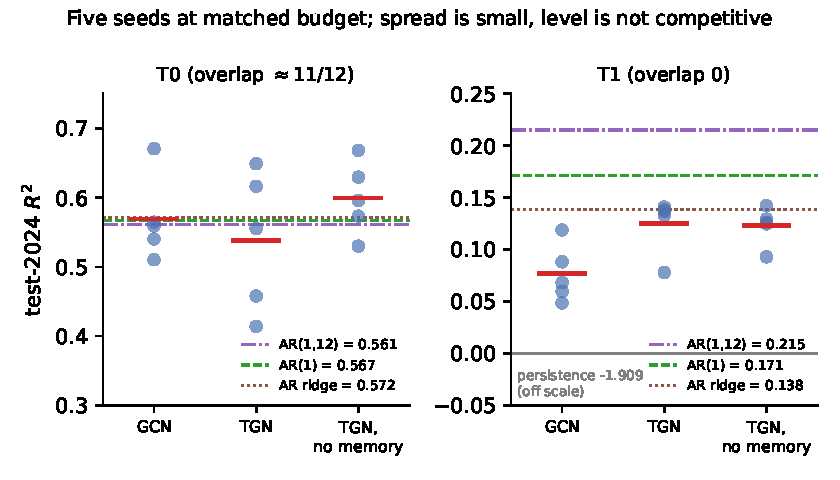
\includegraphics[width=0.85\columnwidth]{graph_seeds.pdf}
\caption{Test-2024 $R^2$ of each of five seeds (dots) and their mean (bar) for the three graph models at the matched budget (80 epochs, patience 15). Dash-dot: AR(1,12); dashed: univariate AR(1); dotted: three-feature AR ridge. On T1 no seed of any graph model reaches the AR(1), let alone the AR(1,12). Source: \texttt{results/phase07/graph\_convergence\_\{T0,T1\}.csv}.}
\label{fig:seeds}
\end{figure}

\subsection{F4. Exogenous channels add nothing under either construction}

After rebuilding news (per-country $z$ and surprise), weather (seasonal temperature $z$), and GSCPI (change and lag) from raw files, none improves on the AR baseline under both targets (Table~\ref{tab:exog}). News and GSCPI lower $R^2$ on T0 and on T1; weather moves it by less than $0.01$ on either target, which is within noise. This is the direct rebuttal to fusion papers in Table~\ref{tab:litsynth} that treat those channels as incremental signal without an autoregressive control.

\begin{table}[t]
\centering
\caption{Tuned-ridge test $R^2$ after adding re-engineered exogenous groups to the three-feature AR. Canonical rows.}
\label{tab:exog}
\footnotesize
\begin{tabular}{l cc}
\toprule
\textbf{Channel} & \textbf{T0} & \textbf{T1} \\
\midrule
AR baseline & $0.572$ & $0.138$ \\
{}+ news & $0.338$ & $0.008$ \\
{}+ weather & $0.570$ & $0.144$ \\
{}+ GSCPI & $0.501$ & $-0.023$ \\
{}+ all & $0.464$ & $-0.054$ \\
\bottomrule
\end{tabular}
\end{table}

\subsection{F5. Single-split evaluation reports regime}
\label{sec:roll}

A zero-parameter persistence rule on T0 swings from $R^2=-0.169$ to $+0.708$ across expanding six-month origins (Fig.~\ref{fig:origins}, Table~\ref{tab:origins}). T1 persistence is stably anti-predictive. The 2024 headline $0.648$ is a high-persistence regime, not a property of the model class.

The fitted models tell the same story once they are refit at each origin instead of scored on 2024 alone (Table~\ref{tab:rollmodels}). For each six-month block, the six preceding months are the validation window and all earlier months from 2021-12 are training; blocks with fewer than eight training months are skipped, which leaves four. On T1 the AR(1,12) is the best tabular model in all four blocks (mean $R^2$ $0.206$), ahead of the AR(1) ($0.155$), the three-feature ridge ($0.148$), and the random forest ($0.099$). The AR(1) and the ridge trade places from block to block, so the single-year gap between them is not stable. On T0 the ordering follows the regime: the ridge leads in three blocks and zero-parameter persistence in the fourth. Graph models are not refit per origin because of their cost.

\begin{table}[t]
\centering
\caption{Tabular models refit at each expanding origin, $R^2$ on six-month T1 blocks. Validation is the six months before each block; training is all earlier months from 2021-12. Source: \texttt{results/phase08/rolling\_origin\_models.csv}.}
\label{tab:rollmodels}
\footnotesize
\begin{tabular}{l r r c ccc c}
\toprule
\textbf{Block} & $n$ & \textbf{Train mo.} & \textbf{Persistence} & \textbf{AR(1)} & \textbf{AR(1,12)} & \textbf{3-feat.\ ridge} & \textbf{RF} \\
\midrule
2023-02..07 & 108 & 8 & $-1.872$ & $0.146$ & $\mathbf{0.213}$ & $0.164$ & $0.060$ \\
2023-08..2024-01 & 106 & 14 & $-1.672$ & $0.120$ & $\mathbf{0.172}$ & $0.123$ & $0.061$ \\
2024-02..07 & 102 & 20 & $-1.855$ & $0.146$ & $\mathbf{0.195}$ & $0.189$ & $0.186$ \\
2024-08..12 & 68 & 26 & $-2.213$ & $0.209$ & $\mathbf{0.245}$ & $0.116$ & $0.089$ \\
\midrule
Mean & & & $-1.903$ & $0.155$ & $\mathbf{0.206}$ & $0.148$ & $0.099$ \\
\bottomrule
\end{tabular}
\end{table}

\begin{figure}[t]
\centering
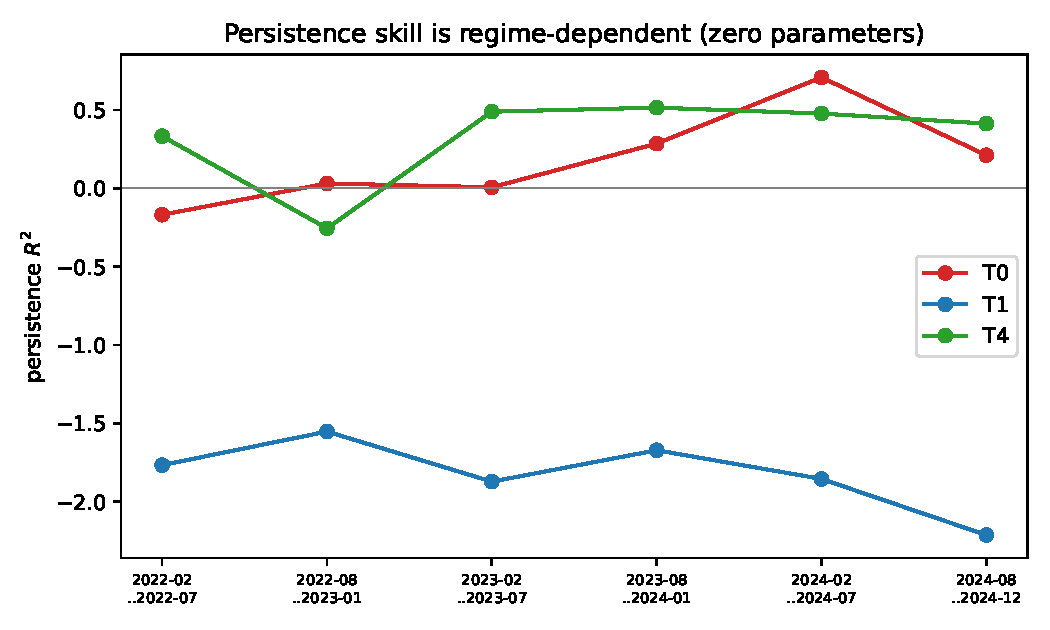
\includegraphics[width=\columnwidth]{per_origin_persistence.pdf}
\caption{Persistence $R^2$ by expanding origin. Zero parameters fitted.}
\label{fig:origins}
\end{figure}

\begin{table}[t]
\centering
\caption{Per-origin persistence $R^2$, six-month evaluation blocks.}
\label{tab:origins}
\footnotesize
\begin{tabular}{l r rrr}
\toprule
\textbf{Window} & $n$ & T0 & T1 & T4 \\
\midrule
2022-02..07 & 108 & $-0.169$ & $-1.767$ & $0.332$ \\
2022-08..2023-01 & 108 & $0.031$ & $-1.553$ & $-0.256$ \\
2023-02..07 & 108 & $0.006$ & $-1.872$ & $0.489$ \\
2023-08..2024-01 & 106 & $0.285$ & $-1.672$ & $0.514$ \\
2024-02..07 & 102 & $0.708$ & $-1.855$ & $0.477$ \\
2024-08..12 & 68 & $0.211$ & $-2.213$ & $0.413$ \\
\bottomrule
\end{tabular}
\end{table}

%--------------------------------------------------------------
\section{Implications}
\label{sec:impl}

A reporting floor for this task is short. (i)~State the target's overlap fraction, or the number of months shared with its own lag. (ii)~Report persistence, zero, and an expanding-origin sweep before any fitted model. (iii)~If the use case is alerting, say so and fix the flagged rate; do not inherit a $\tau$ from a rolling-median label.

F1 on this panel is the known overlapping-observations bias~\citep{ref29,ref32}, measured here on trade flows built from public data rather than on asset returns. The scientific claim is not that trade is unpredictable. Year-over-year $H_{12}$ is predictable because it overlaps. One-step growth is weakly mean-reverting with an annual echo, and otherwise unpredictable from the channels this literature usually ships.

%--------------------------------------------------------------
\section{Limitations}
\label{sec:limits}

The test set is small ($n=193$ on T0; $n=187$ on T1). One India-centred country universe (India and its 17 largest partners for a single consumer-goods basket) and a four-year span bound external validity. Seventeen (T1) or eighteen (T0) clusters are few for cluster-robust inference; we report three $p$-values and do not pretend DM-HLN is correctly specified. Graph claims are scoped to a matched compute budget (80 epochs, five seeds, CPU, per-node TGN loops). T1 classification is omitted. The horizon sweep is one panel. Hyperparameter search and all sixteen reported test pairs (Tables~\ref{tab:sig} and~\ref{tab:seasonal}) are unadjusted for multiplicity. Four pairs clear $0.05$ on the wild bootstrap. AR(1) versus zero, at $0.001$, would survive a Bonferroni correction over the sixteen. The other three would not: the three-feature ridge versus zero ($0.043$), the AR(1,12) versus the AR(1) ($0.037$), and the AR(1,12) versus the GCN ensemble ($0.022$). The lag-12 gain is therefore best read as consistent across origins but not individually decisive. Every other pair is a tie by a wide margin. Canonicalization itself showed that single-seed early-stopped graphs overfit evaluation protocol; we cannot rule out that a larger search would move the graph means, only that it did not under the budget we can defend. Finally, a live scoring pipeline (LLM, news and weather extractors feeding the same seven-feature schema) exists alongside this corpus, but its extractors have not been validated against the fused historical fields, so it is excluded from every result reported here.

%--------------------------------------------------------------
\section{Conclusion}
\label{sec:concl}

Overlapping-window targets manufacture forecasting skill. That mechanism is known in financial econometrics~\citep{ref29,ref32}; on this panel the manufactured part is most of the number. What remains after the overlap is removed is the target's own serial structure, an autoregression on its lags 1 and 12 at $R^2=0.215$ (lag 1 alone: $0.171$), which no feature, channel, or graph exceeds. Stating overlap and reporting persistence should be preconditions for reporting skill on trade disruption, and likely on any monthly series whose target is a trailing-window deviation.

\section*{Data and Code Availability}

Corpus, target family, canonical numbers (\texttt{results/canonical\_numbers.csv}), figures, and reproduction scripts are in the accompanying anonymized artifact (\texttt{artifact/DATASHEET.md}, \texttt{reproduce.sh}). The horizon sweep behind Table~\ref{tab:targets} and Fig.~\ref{fig:overlap} is \texttt{results/phase06/horizon\_sweep.csv}; every $p$-value in Table~\ref{tab:sig} is written by \texttt{dataset/dm\_tests.py} to \texttt{results/phase06/dm\_tests.csv}. Graph predictions used in Tables~\ref{tab:sig} and~\ref{tab:seasonal} are the five-seed ensembles in \texttt{results/phase07/}. The lag-12 tests and the rolling-origin refits are written by \texttt{dataset/seasonal\_and\_rolling.py} to \texttt{results/phase08/}. The public URL will be inserted at submission; this draft does not claim a release.

\clearpage
\appendix
\section{Literature mapping}
\label{app:lit}

%--------------------------------------------------------------
\begin{table}[!h]
\centering
\caption{Reviewed work by data, time treatment, structure, headline result, and main limit. Figures are those reported by each paper on its own data and are not comparable across rows. Limitations are those the authors state where they state one; otherwise they are our reading.}
\label{tab:litsynth}
\tiny
\begin{tabular}{L{1.35cm} L{1.85cm} L{1.7cm} L{1.55cm} L{2.15cm} L{2.15cm}}
\toprule
\textbf{Work} & \textbf{Data} & \textbf{Temporal treatment} & \textbf{Structure} & \textbf{Headline result} & \textbf{Principal limitation} \\
\midrule
\citet{ref35} & Aerospace multi-tier SC, $\approx$500k deliveries, 2011--2016 & Random 80:20 hold-out per supplier; stratified 5-fold CV & SVM (RBF) and decision tree & Late delivery; tree costs 5\% recall, 37\% average precision vs SVM; Zero-Rule baseline & Mainly date-derived features; 23\% late (imbalance) \\
\citet{ref36} & OEM ERP, 232,912 orders, 351 suppliers, one year & No split reported & RF, LR, SVM, KNN (tabular) & Late orders: RF precision 0.83, recall 0.78 vs 0.157 weighted guess & Class imbalance; internal data only; single case study \\
\citet{ref2} & DataCo Global SC data & None & None (tabular) & 85.4\% accuracy vs 84.1\% XGBoost & 1.3 pt gain for three-model ensemble; no split reported \\
\citet{ref5} & Synthetic, 200 nodes & Static snapshot & Multi-head GAT & $F_1$ 0.9630; 0.7143 without graph & Synthetic generator; static structure \\
\citet{ref6} & FMCG, public, Jan--Aug 2023 & 8:2 temporal split & Homogeneous and heterogeneous temporal GNN & Demand mean diff.\ 304.68 (LSTM) to 251.23; RMSE 30.78 to 26.24 (HTGNN) & Short temporal scope \\
\citet{ref7} & Carbon Monitor and IEA, $>$500 firms, 2015--2022 & Fiscal-year labels; episodic few-shot sampling & Adaptive V2E plus GCN & AUPRC 0.850, FNR 0.080, WAC 45 & $O(N^2)$ edge inference; cold start \\
\citet{ref10} & Wikipedia, Reddit, Twitter & Continuous-time events & Per-node memory plus attention & State of the art continuous-time link prediction & Not applied to supply chains \\
\citet{ref11} & 13 benchmark datasets & Continuous-time sequences & Patching transformer, no memory & State of the art on most of 13 datasets; unified library (DyGLib) & Not applied to supply chains \\
\citet{ref16} & Changhong SC (industry partner) & Static snapshot & HKTGNN (GEE + GIN) & $F_1$ 83.13\% vs 74.47\% KTGNN, 72.30\% GATv2 & Random 7:1:2 split; no temporal holdout \\
\citet{ref13} & Wikipedia, Reddit, Walmart grocery & Continuous-time events & TGAT & Inductive AP 84.99\% (industrial) & Stateless; no node memory \\
\citet{ref14} & Various public & Survey & Survey & Taxonomy of dynamic GNNs & History-only EdgeBank baseline can do well; benchmarks may not separate models \\
\citet{ref17} & Typhoon Soulik, Korean SC & Multi-stream snapshots & Causal, route, application graphs & Advance shipment under disruption & Requires prior causal-impact analysis \\
\citet{ref18} & CSMAR Auto SC & Static snapshot & EGAT with contrastive learning & Accuracy 0.9667, $F_1$ 0.8903 & Sparse networks limit high-order aggregation \\
\citet{ref21} & News articles & None (per document) & LLM binary classifier (SCREWS) & Temperature 0.4--0.7 optimal; Top-$p$ weak & Binary labels, not numeric features; single model \\
\citet{ref23} & Auto, pharma, electronics networks & Weekly/daily snapshots + LSTM & Physics-informed GNN & 23\% error reduction; $F_1$ 0.87 vs 0.71 & Only flow and capacity constraints; disruption types treated uniformly \\
\bottomrule
\end{tabular}
\end{table}

\clearpage
\section{Denominator ablations of T0}
\label{app:t2t3}

Table~\ref{tab:t2t3} reports the two denominator ablations referenced in Section~\ref{sec:corpus}. Let $\mathrm{med}_{12}$ be the median of $V_{T-11..T}$. T2 replaces the rolling denominator with $B_v$, the per-country mean flow over the training window, so the denominator is constant in $T$ but the numerator $V_{T+1}-\mathrm{med}_{12}$ is still a level. T3 keeps the T0 target and rebuilds only the lagged-contraction feature with a median over months $\le T-12$, so feature and target denominators are disjoint. Neither ablation removes the apparent skill; only T1, which removes the level, does. The AR model is the three-feature ridge of Table~\ref{tab:ladder}, with $\alpha$ tuned on 2023 validation; for T3 its lagged-contraction feature is the disjoint-denominator version.

\begin{table}[!h]
\centering
\caption{Denominator-overlap ablations, test 2024 $R^2$. Persistence is the previous-month value of the same target; $n$ is the number of test rows with a valid target. Source: \texttt{results/canonical\_numbers.csv}.}
\label{tab:t2t3}
\footnotesize
\begin{tabular}{l l l c cc}
\toprule
\textbf{Id} & \textbf{Definition} & \textbf{Denominator overlap} & $n$ & \textbf{AR ridge (3 feat.)} & \textbf{Persistence} \\
\midrule
T0 & $(V_{T+1}-\mathrm{med}_{12})/\mathrm{med}_{12}$ & $11/12$ shared & 193 & $0.572$ & $0.648$ \\
T1 & $\log(V_{T+1}/V_T)$ & none & 187 & $0.138$ & $-1.909$ \\
T2 & $(V_{T+1}-\mathrm{med}_{12})/B_v$ & constant in $T$ & 198 & $0.565$ & $0.560$ \\
T3 & T0 target, disjoint feature denominator & disjoint & 193 & $0.482$ & $0.648$ \\
\bottomrule
\end{tabular}
\end{table}

\clearpage
\begin{thebibliography}{99}

\bibitem[Baryannis et~al.(2019)]{ref35} Baryannis, G., Dani, S., and Antoniou, G. (2019). Predicting supply chain risks using machine learning: The trade-off between performance and interpretability. \emph{Future Generation Computer Systems}, 101, 993--1004.

\bibitem[Brintrup et~al.(2020)]{ref36} Brintrup, A., Pak, J., Ratiney, D., Pearce, T., Wichmann, P., Woodall, P., and McFarlane, D. (2020). Supply chain data analytics for predicting supplier disruptions: a case study in complex asset manufacturing. \emph{International Journal of Production Research}, 58(11), 3330--3341.

\bibitem[Jin(2024)]{ref2} Jin, T. (2024). Integrated machine learning for enhanced supply chain risk prediction. In \emph{Proc. 8th Int. Conf. Electronic Information Technology and Computer Engineering (EITCE)}, Haikou, China. ACM.

\bibitem[Kayalvizhi et~al.(2025)]{ref5} Kayalvizhi, S., Jothi, D.~S.~J., Devi, T., and Brijet, Z. (2025). Graph neural network-based predictive modeling for enhanced supply chain resilience against multi-modal disruptions. \emph{Journal of Information Systems Engineering and Management}, 10(33s).

\bibitem[Wang and Sun(2026)]{ref7} Wang, Y. and Sun, Y. (2026). Low-carbon supply chain logistics risk prediction using meta-learning-based graph convolutional network on prototype space. \emph{Scientific Reports}, 16, 2352.

\bibitem[Petrova and Hughes(2025)]{ref23} Petrova, S. and Hughes, M. (2025). Physics-informed graph neural networks for supply chain disruption prediction and mitigation. \emph{Frontiers in Applied Physics and Mathematics}, 2(1), 130--145.

\bibitem[Hansen and Hodrick(1980)]{ref29} Hansen, L.~P. and Hodrick, R.~J. (1980). Forward Exchange Rates as Optimal Predictors of Future Spot Rates: An Econometric Analysis. \emph{Journal of Political Economy}, 88(5), 829--853.

\bibitem[Richardson and Stock(1989)]{ref30} Richardson, M. and Stock, J.~H. (1989). Drawing inferences from statistics based on multi-year asset returns. \emph{Journal of Financial Economics}, 25(2), 323--348.

\bibitem[Valkanov(2003)]{ref31} Valkanov, R. (2003). Long-horizon regressions: theoretical results and applications. \emph{Journal of Financial Economics}, 68(2), 201--232.

\bibitem[Boudoukh et~al.(2008)]{ref32} Boudoukh, J., Richardson, M., and Whitelaw, R.~F. (2008). The Myth of Long-Horizon Predictability. \emph{Review of Financial Studies}, 21(4), 1577--1605.

\bibitem[Diebold and Mariano(1995)]{ref28} Diebold, F.~X. and Mariano, R.~S. (1995). Comparing Predictive Accuracy. \emph{Journal of Business \& Economic Statistics}, 13(3), 253--263.

\bibitem[Harvey et~al.(1997)]{ref33} Harvey, D., Leybourne, S., and Newbold, P. (1997). Testing the equality of prediction mean squared errors. \emph{International Journal of Forecasting}, 13(2), 281--291.

\bibitem[Cameron et~al.(2008)]{ref34} Cameron, A.~C., Gelbach, J.~B., and Miller, D.~L. (2008). Bootstrap-Based Improvements for Inference with Clustered Errors. \emph{The Review of Economics and Statistics}, 90(3), 414--427.

\bibitem[Wasi et~al.(2025)]{ref6} Wasi, A.~T., Islam, M.~S., Akib, A.~R., and Bappy, M.~M. (2025). Graph neural networks in supply chain analytics and optimization: Concepts, perspectives, dataset and benchmarks. arXiv:2411.08550v2.

\bibitem[Zheng et~al.(2024)]{ref14} Zheng, Y., Yi, L., and Wei, Z. (2024). A survey of dynamic graph neural networks. \emph{Frontiers of Computer Science}.

\bibitem[Park and Lee(2025)]{ref17} Park, S. and Lee, H. (2025). Predictive supply chain disruption control framework using causal network-based multi-stream deep learning. \emph{Computers \& Industrial Engineering}, 207, 111312.

\bibitem[Zhou et~al.(2023)]{ref16} Zhou, Z., Bi, K., Zhong, Y., Tang, C., Li, D., Ying, S., and Wang, R. (2023). HKTGNN: Hierarchical Knowledge Transferable Graph Neural Network-based Supply Chain Risk Assessment. In \emph{Proc. IEEE Int. Conf. Parallel \& Distributed Processing with Applications, Big Data \& Cloud Computing, Sustainable Computing \& Communications, Social Computing \& Networking (ISPA/BDCloud/SocialCom/SustainCom)}, Wuhan, China, 772--782. IEEE.

\bibitem[K\"uhl et~al.(2026)]{ref21} K\"uhl, L., Wieth\"olter, J., and Dircksen, M. (2026). Leveraging AI for accurate supply chain risk classification: optimizing the operational parameter space of LLMs. \emph{The International Journal of Logistics Management}, 37(3), 730--754.

\bibitem[Rossi et~al.(2020)]{ref10} Rossi, E., Chamberlain, B., Frasca, F., Eynard, D., Monti, F., and Bronstein, M. (2020). Temporal graph networks for deep learning on dynamic graphs. arXiv:2006.10637.

\bibitem[Xu et~al.(2020)]{ref13} Xu, D., Ruan, C., Korpeoglu, E., Kumar, S., and Achan, K. (2020). Inductive Representation Learning on Temporal Graphs. In \emph{International Conference on Learning Representations (ICLR)}.

\bibitem[Yu et~al.(2023)]{ref11} Yu, L., Sun, L., Du, B., and Lv, W. (2023). Towards better dynamic graph learning: New architecture and unified library. In \emph{Advances in Neural Information Processing Systems (NeurIPS)}.

\bibitem[Liu et~al.(2025)]{ref18} Liu, Y., Liu, S., and Lu, Y. (2025). Supply chain financial risk assessment: A modified graph attention neural network. \emph{Finance Research Letters}, 86, 108285.

\end{thebibliography}

\end{document}